% ~ 6 pages
\chapter{The ATLAS Experiment at the Large Hadron Collider}
\label{chap:atlas}

The LHC at CERN is a symmetric proton--proton and heavy ion collider, supplying
collision events to four major experiments: ATLAS, CMS, ALICE and LHCb. In
proton--proton operation, bunches of protons are crossed at the interaction
points located inside of the experiments with a peak bunch crossing rate
of~\SI{40}{\mega\hertz}~\cite{lhc}. With a proton beam energy of \SI{6.5}{\TeV}
during Run 2 of the LHC, the collisions take place at a center-of-mass energy of
\SI{13}{\TeV} with a peak instantaneous luminosity of
\SI{1.4e34}{\per\square\centi\metre\per\second} reached during the 2016 $pp$
data taking period~\cite{lhc_2016_report}.

\section{The ATLAS Detector}
\label{sec:atlas}

The ATLAS detector~\cite{atlas_detector} is a multipurpose particle detector
experiment at the LHC. An overview of the detector is given in
Figure~\ref{fig:atlas_detector}. Due to its cylindrical geometry, it provides
almost $4\pi$~coverage of the interaction point and forward-backward symmetry.
Specialised detector systems are arranged in concentric layers around the beam
axis, enabling to measure and reconstruct a multitude of physics objects, e.g.\
photons, muons, taus and .

\begin{figure}[htb]
  \centering
  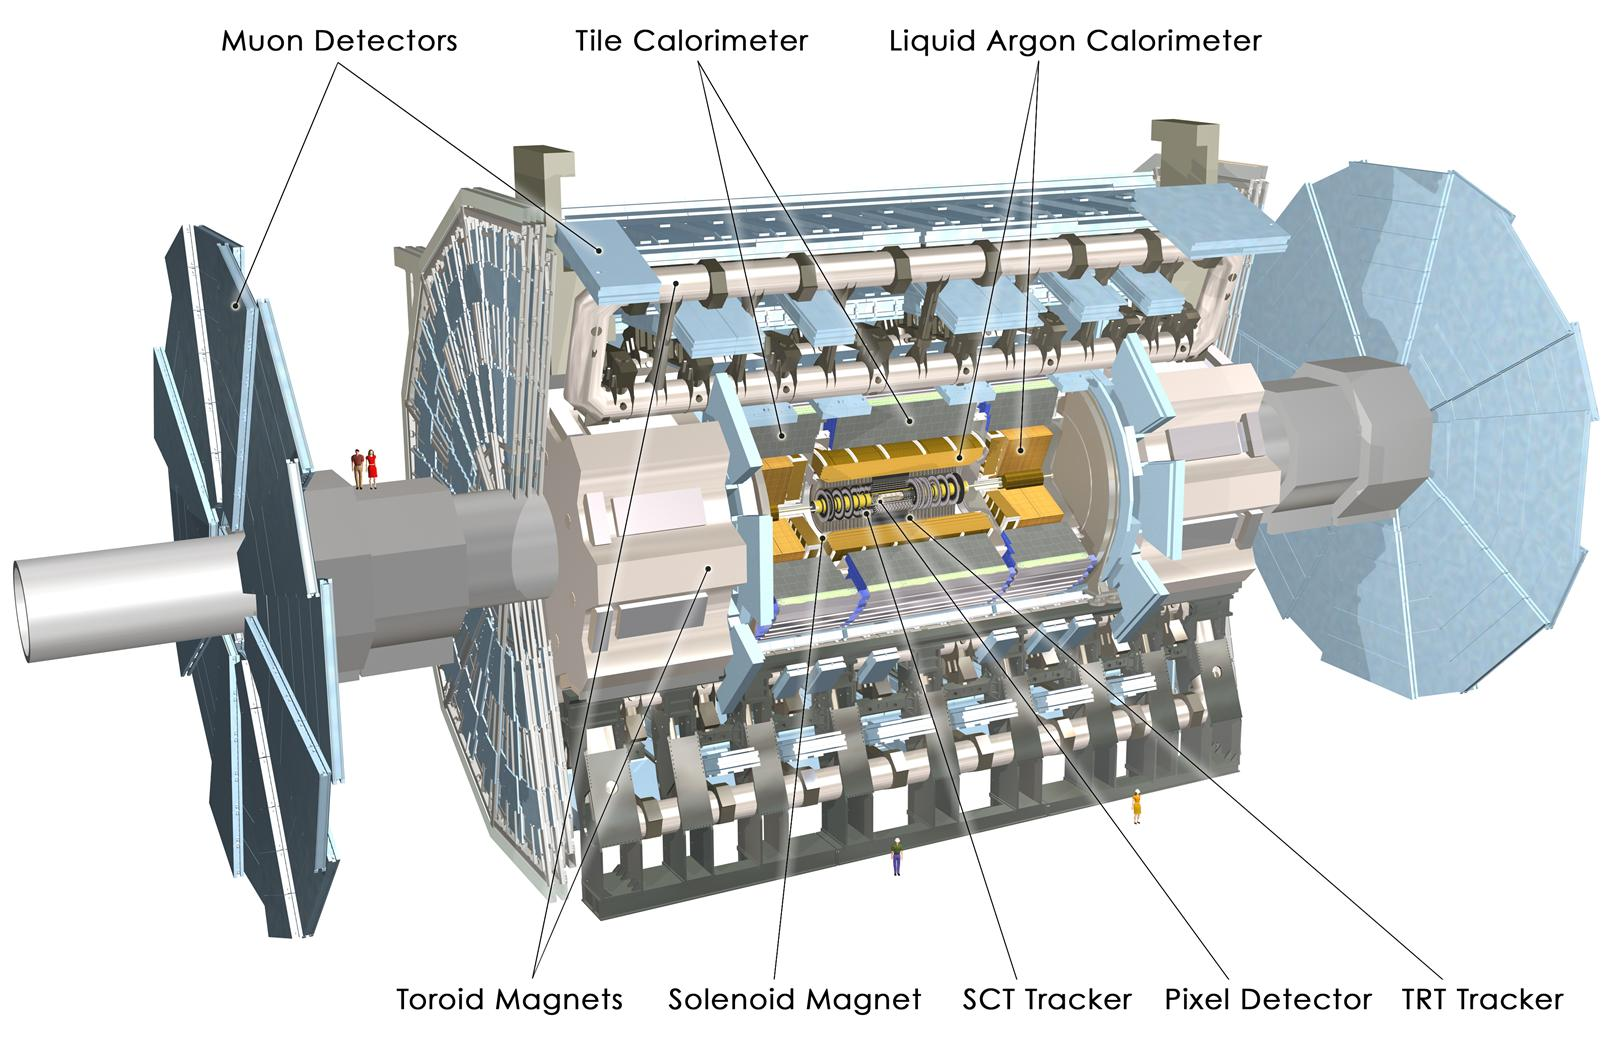
\includegraphics[width=0.8\textwidth]{./figures/atlas/overview.jpg}
  \caption{Overview of the ATLAS detector~\cite{atlas_detector}.}
  \label{fig:atlas_detector}
\end{figure}


\begin{description}
\item[Inner Detector] The Inner Detector (ID) consists of several layers of
  pixel detectors, silicon microstrip detectors and straw tubes of the
  Transition Radiation Tracker (TRT). It allows to reconstruct space points of
  charged particles at different radii, which are used to reconstruct tracks and
  to measure the transverse momenta from the curvature in the \SI{2}{\tesla}
  axial magnetic field. The TRT offers electron identification via
  high-threshold hits originating from transition radiation created by electrons
  crossing the straw tube material.

\item[Calorimeter] The calorimeter system allows the energy measurement of
  electrons, photon and hadrons. It consists of an electromagnetic calorimeter
  with high granularity to measure energy depositions of electrons and photons
  and a hadronic calorimeter for measuring hadrons.

\item[Muon Spectrometer] Three layers of tracking chambers in the magnetic field
  of an air-core toroid outside of the calorimeter system, are used to measure
  the momentum of muons.

\item[Trigger System] The peak event rate of \SI{40}{\mega\hertz}, mostly
  consisting of events not of immediate interest for physics research, needs to
  be reduced in the trigger system to match the limited throughput of the data
  acquisition systems. The trigger system is divided into three levels: L1, L2
  and the event filter, which successively reduce the rate while having access
  to detector information of increasing granularity. The rate after the event
  filter allows moving the events to permanent storage for later analysis.
\end{description}


\section{Coordinate System}
\label{sec:atlas_coord_sys}

In the ATLAS experiment a right-handed coordinate system is used to describe
positions in the detector. The origin of the coordinate system is located at the
nominal interaction point, with the $z$-axis pointing in beam direction, the
$x$-axis pointing towards the center of the LHC ring and the $y$-axis pointing
upwards. The $x$ and $y$ axes span the transverse plane. Cylindrical
coordinates~$(r, \varphi, z)$ with the azimuthal angle $\varphi$ or spherical
coordinates $(r, \varphi, \theta)$ with the polar angle~$\theta$ with respect to
the beam pipe are commonly used.

Due to the unknown longitudinal momentum of colliding partons in longitudinal
direction, the momentum of final state particles only balances in the transverse
plane. Therefore, transverse quantities for momentum and energy are defined as
\begin{align*}
  p_\text{T} &= |\vec{p}| \sin\theta & E_\text{T} &= E \sin{\theta} \eqcomma
\end{align*}
where ABC. Moreover, the unknown boost along the $z$-axis leads to the definition of
the pseudorapidity
\begin{align*}
  \eta &= -\ln\left[\tan\left( \frac{\theta}{2} \right) \right] \eqcomma
\end{align*}
such that differences in pseudorapidity are Lorentz-invariant in the massless
limit. As a result, the Lorentz-invariant angular distance between two
reconstructed objects is given by
\begin{align*}
  \Delta R &= \sqrt{(\Delta\eta)^2 + (\Delta\varphi)^2} \eqcomma
\end{align*}
where $\Delta \eta$ and $\Delta \varphi$ are the differences in pseudorapidity
and azimuthal angle, respectively.


\subsection{Tracking System}
\label{sec:atlas_tracking}

\begin{figure}[ht]
  \centering
  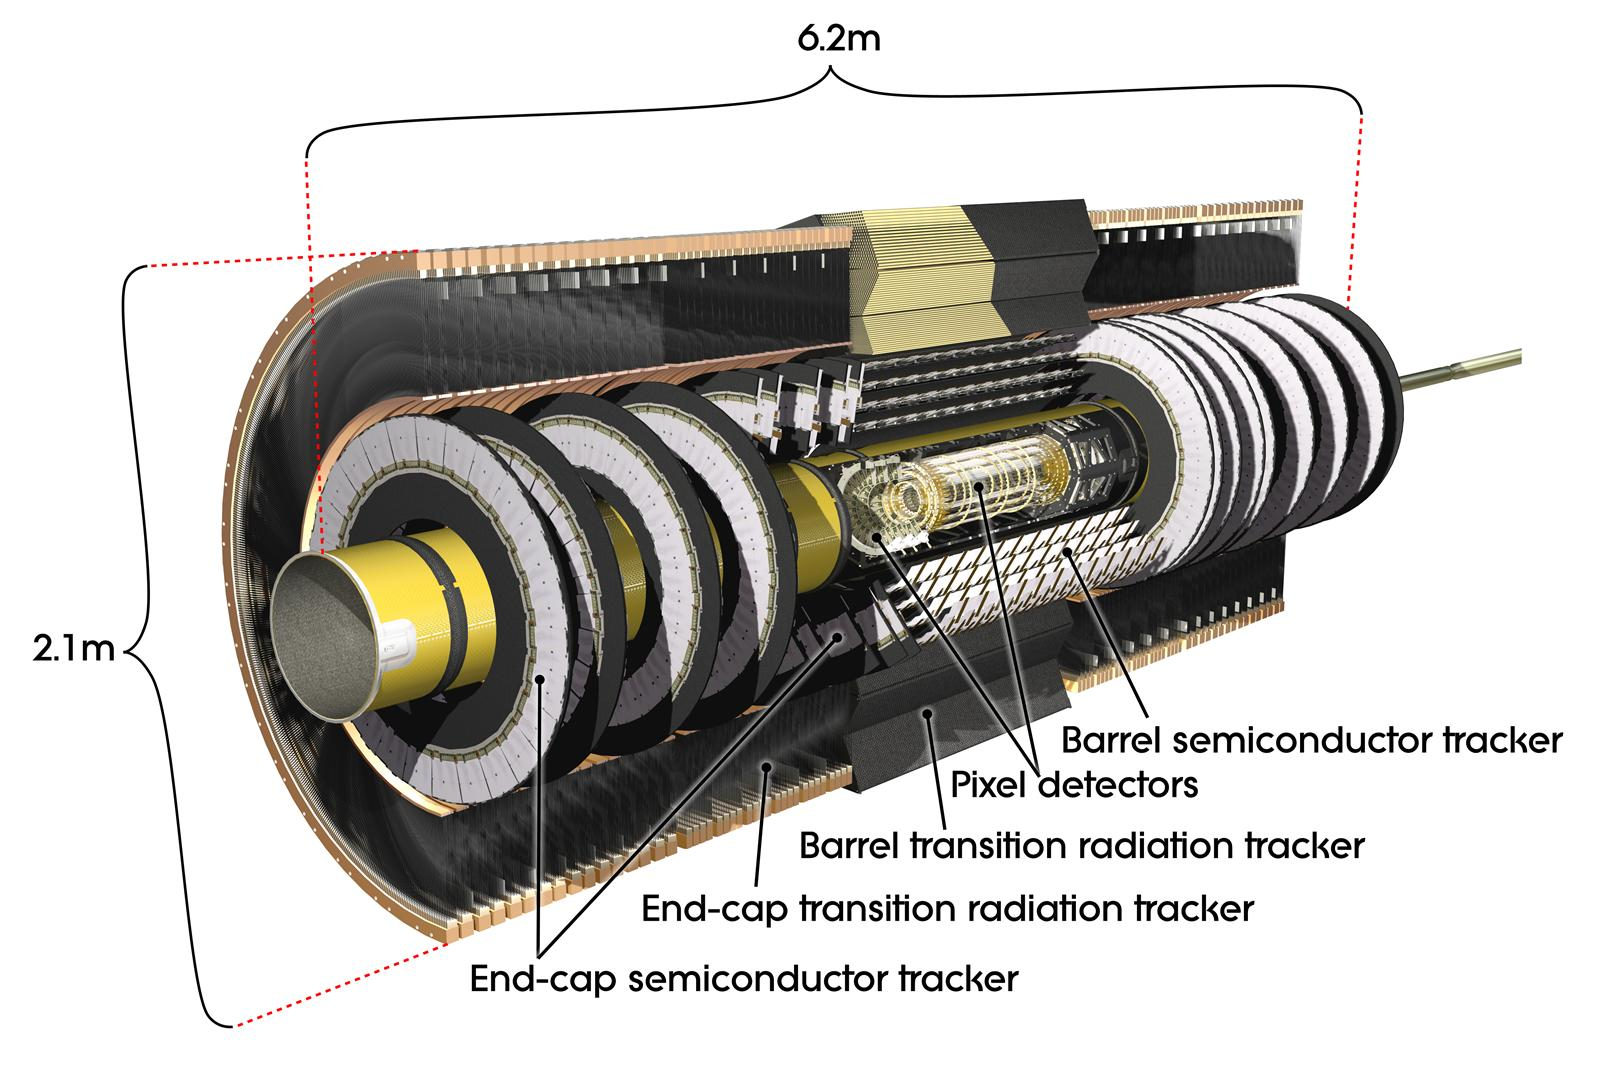
\includegraphics[width=0.75\textwidth]{./figures/atlas/inner_detector.jpg}
  \caption{ATLAS inner detector\cite{indet_fig} also in \cite{atlas_detector}}
  \label{fig:atlas_indet}
\end{figure}

\todo[inline]{Name this 'Inner Detector'?}
\todo[inline]{Introduce abbrev.\ ID}
\todo[inline]{Introduce abbrev.\ IBL}
\todo[inline]{Define impact parameter: $d_0$ and $z_0$.}
\todo[inline]{Define perigee}
% See \url{https://twiki.cern.ch/twiki/bin/view/AtlasProtected/InDetTrackingDC14#Impact_parameters_z0_d0_definiti}

Coverage to $|\eta| < 2.5$

\todo[inline]{Find primary sources on this stuff!}
\begin{itemize}
\item Track \& vertex reconstruction
\item Charged particles provide hits in ID
\item High spacial resolution to reconstruct tracks in dense environments
  (number of tracks per event -- 200? -- check this)
\item Solenoid field with \SI{2}{\tesla}
\item Secondary vertex reconstruction (B-layer -- this is important, Pixel, SCT)
\item TRT -- 'continuous' tracking (what is this?) and distinction between
  electrons and hadrons using transition-radiation
\item ID acceptance $|\eta| < \num{2.5}$
\item Split into barrel and two endcap regions
\item Pixel: Three barrel layers, three endcap layers each (and 1 layer IBL).
  Pixel detector in 'Pixel Support Tube' to allow exchange of elements in case
  of radiation damage. Inner Radius \SI{4.2}{\centi\metre} and outer radius
  \SI{25}{\centi\metre}.
\item The layer after the IBL is called B-layer!
\item IBL \cite{ibl_tdr}: Improve B-tagging when modules in the remaining pixel layers fail;
  Tracking inefficiencies at high pileup affects B-layer needs redundancy;
  Better impact parameter reconstruction improves vertexing and b-tagging
\item Pixel layers segmented in $r\varphi$ and $z$. Single pixel
  \SI{50}{\micro\metre} in $r\varphi$ and \SI{400}{\micro\metre} in $z$
\item Silicon strip detectors (four layers) in support structure with radius of
  about \SI{55}{\centi\metre}
\item SCT strip detectors \SI{15}{\micro\metre} $r\varphi$ and
  \SI{70}{\micro\metre} $z$ resolution
\item TRT: Barrel region $|\eta| < \num{0.5}$, on average a track causes 36
  hits; Resolution decreases with pile-up
\end{itemize}

\subsection{Calorimeter System}
\label{sec:atlas_calo}

\todo[inline]{Topoclustering}
\todo[inline]{Define what a moment is}
\todo[inline]{EM and LC scale}
\todo[inline]{Introduce nomenclature: strip layer, EM1, EM2, EM3, HAD}

Coverage:

EM LAr covers $|\eta|< 3.2$

Scintillator-tile in~$|\eta| < 1.7$

End-caps hadronic $|\eta| > 1.5$ also LAr coverage to $|\eta| = 4.9$

\begin{figure}[ht]
  \centering
  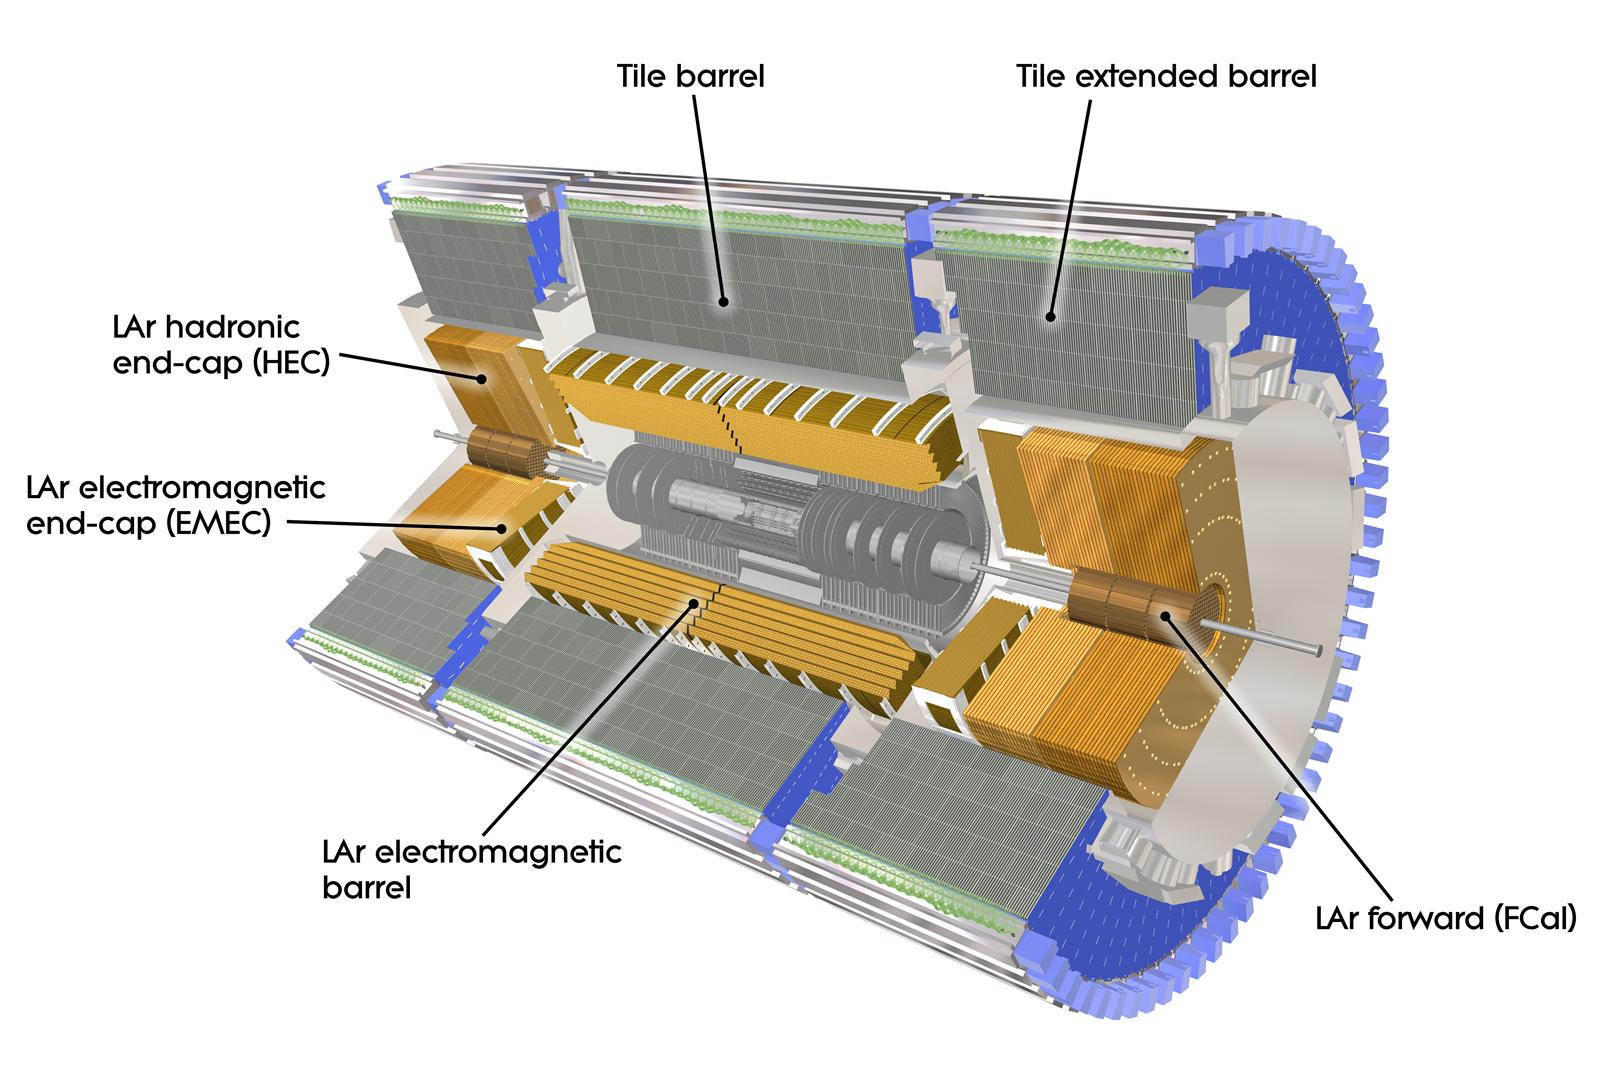
\includegraphics[width=0.8\textwidth]{./figures/atlas/calorimeter.jpg}
  \caption{ATLAS calorimeter\cite{calo_fig} also in \cite{atlas_detector}}
  \label{fig:atlas_indet}
\end{figure}



\begin{itemize}
\item LHC (brief)

\item ATLAS
  \begin{itemize}
  \item Overview (Design goals) \\
    brief: Beam Line, Inner Detector \& Solenoid, Calorimeter, Muon System \&
    Toroid, Trigger

  \item Nomenclature (Coordinate system, Pseudorapidity, $\Delta R$,
    $p_\mathrm{T}$)

  \item Inner detector / Tracker (and why they are important for taus)
    \begin{itemize}
    \item Pixel, IBL
    \item SCT
    \item TRT
    \item  Transverse Momentum Resolution, Vertex \& Secondary Vertex
      reconstruction, Impact Parameter Resolution, $\eta$-Coverage
    \end{itemize}

  \item Calorimeter (and why they are important for taus)
    \begin{itemize}
    \item Presampler, LAr (EM1 - EM3), Had (Tile, LAr)
    \item Cell sizes, $\eta$-Coverage, Thickness $X_0$ / $\lambda$,
      Energy Resolution vs. $E$
    \item Topoclusters \& Cluster moments
    \end{itemize}

  \end{itemize}
\end{itemize}

%%% Local Variables:
%%% mode: latex
%%% TeX-master: "mythesis"
%%% End:
